\subsection{Use Case - Edinburgh Cancer Data Gateway}
\label{sec:useCase}

\noindent
We are developing a dashboard to help oncologists observe, monitor, and analyse the condition of their patients over time. It can also be used to analyse the effect of different chemotherapy treatments when given to patients with similar characteristics, and consequently influence future decisions to improve the well-being and survival rate of patients. Our ultimate aim is to build a \emph{toxicity predictor} (Figure~\ref{fig:USTANDiagram}) to predict the toxicity of chemotherapy treatments based on history and feedback from patients.
%
\begin{figure}[t!]
    \centering
    \includegraphics[width=0.45\textwidth]{images/USTANUseCase2.png}
    \caption{Toxicity Predictor for Breast Cancer Treatment}
    \label{fig:USTANDiagram}
\end{figure}
%
\begin{figure}[t!]
    \centering %[angle=-90,width=0.45\textwidth]
    \includegraphics[width=0.45\textwidth]{images/USTANDataGateway.png}
    \caption{Database Structure for Training the Toxicity Predictor Model}
    \label{fig:ECG}
\end{figure}
Figure~\ref{fig:ECG} shows the data structure we use for training the toxicity predictor. We extracted data 
%during the initial step 
for training the machine learning models from three main databases (i.e., Chemocare, Trak, and Oncology DB) within the Edinburgh Cancer Centre (ECC). The data contains the information on treatment cycles, recorded side effects (here, toxicity level), comorbidities, and various observations concerning breast cancer patients for three years (from 2014 to 2016). The extraction has data for 51,661 treatments, of which 13,030 are breast cancer treatments. There are 933 unique patients, and some patients may have two or three different treatments/regimes. Each regime has several cycles ranging from one to more than 50 cycles.
%\sout{(e.g., 85)} {\color{red}[cite: On Predicting the Outcomes of Chemotherapy Treatments in Breast Cancer]}.

%\subsection{Evaluation Framework}

\subsection{Smart Patient Records}
\label{sec:smartPatientRecords}

\begin{table}[h!]
    \centering
    \begin{tabular}{|l|l|l|l|l|}
            \hline \hline
        \textbf{Table name} & \textbf{\# vars} & \textbf{\# num} & \textbf{\# categorical} & \textbf{\# bool} \\
        \hline 
        NDC\_SMR01 & 17 & 3 & 13 & 1 \\
        NDC\_SMR06 & 9 & 2 & 7 & 0 \\
        NDC\_Charlson & 20 & 9 & 5 & 6 \\
        Chemocare\_Toxicity & 17 & 14 & 3 & 0 \\
        Chemocare\_Treatment & 19 & 8 & 11 & 0 \\
        \hline \hline
            \end{tabular}
    \caption{Database Tables Structure from the Edinburgh Cancer Gateway Use Case.}
    \label{tab:useCaseData}
\end{table}

\begin{figure}
    \centering
    \includegraphics[width=45mm]{images/DataVault/smr01_source.png}
    \caption{Example of source table}
    \label{fig:smr01_source}
\end{figure}


%\begin{figure}
%    \centering
 %   \includegraphics[width=80mm]{images/DataVault/DataVault.pdf}
  %  \caption{Example of source table abstracted into Data Vault}
   % \label{fig:dv_smr01}
%\end{figure}

\noindent
The data from %We have received the data from 
the Edinburgh Cancer Gateway %from 5 databases 
(see Table~\ref{tab:useCaseData}), is 
%In turn, each of these were 
abstracted out into their data vault structure. If we take NDC\_SMR01 as the example, we can show it in its original form (see Figure~\ref{fig:smr01_source}). Each of these columns are then examined and classified under one of the following hubs of the Smart Patient Record Data Vault (TPOLE).
%Time, Person, Object, Location, Event. 
Note that not every table will contain elements that fall into every category.

The fields from the NDC\_SMR01 table can be organised into following groupings:
\begin{itemize}
\item \emph{Time}: admission\_ date, discharge\_date, length\_of\_stay;
\item \emph{Person}: sex, age\_in\_years, ethnic\_group, marital\_status, postcode; or
\item \emph{Object}: main\_operation\_a, main\_operation\_b, main\_condition, other\_condition\_1, other\_condition\_2, other\_condition\_3, other\_condition\_4.
\end{itemize}


\noindent These are then broken up into smaller subcategories which will form the satellites of the data vault. In this example, the Object category can be seen to be made up of two sets: one containing details about the operations, and the other containing details about the conditions. %When laid out in the data vault format, the tables now appear as they do in Figure~\ref{fig:dv_smr01}.

\subsection{Data Fabrication}
\label{ssec:DataFabrication}

\noindent
In order to synthesise data, we must pass database table definitions and metadata to the %Data Fabrication Platform (DFP). 
DFP. The metadata itself contains high level information about the data, describing details about its nature, without revealing any of the actual values that make up the source data. In addition, we need to define the rules that the data conforms to, in order to keep the synthetic data as accurate as possible. This might include, for example, the range of values that the data takes and the distribution of these values, as well as any relationships between different data elements. For instance, we might have a column with the appointment date. The metadata would contain the information that it is a date type, the format the date should be stored in, whether it can be null, etc. The rules for it might include that it must be greater than the date of birth for the patient. %IBM will take these rules and plug them into their scripting language, at which point they can produce synthetic data that conforms to these rules.

For the Edinburgh Cancer Gateway use case, we have done some profiling of the real data.
%with a Python package called %"pandas-profiling"\footnote{https://github.com%/pandas-profiling/pandas-profiling}. This %package 
We collected many aspects of the metadata including common, maximum, minimum, and extreme values for each reading. In addition, we derived the distribution of the data value measurements and the correlations between the different values. This profiling can be seen to work 
%as an analogue for the reverse of the data fabrication process,
to derive the required rules to fabricate new data. These rules were then used to synthesise data to be used in the development and evaluation of the SERUMS tool chain.

\subsection{Blockchain}
%{\color{red} [VJ note: Anything we can do here? Show examples (even if they are completely synthetic) of smart contracts related to our setting?]}

%{\color{red} DRAFT to be reviewed Georgios}
%% Add example contract??

The blockchain smart contracts will use the hyper-ledger format (Figure \ref{fig:hyperledger}) and will enable the storage of the preference contract of the patient, the vault of the current active data transport contracts and the valid user contracts of the SERUMS data exchange process.

\begin{figure}
    \centering
    \includegraphics[width=60mm]{images/hyperledger.png}
    \caption{Hyperledger Ecosystem}
    \label{fig:hyperledger}
\end{figure}


\subsection{Authentication}
%{\color{red} [VJ note: Just move some of the stuff from the authentication section here. Can we pull anything from the previous papers?]}

The dual nature of the proposed user authentication scheme allows us to move from "one-size-fits-all" authentication schemes to flexible authentication schemes since users can choose their preferred way to authenticate; either by entering the textual password or the graphical password that represents their single secret. Consider a password creation scenario in which a user chooses a secret derived from his episodic memory, e.g., \emph{Places that we visited in Europe}. In this scenario, the textual password key is based on the articulation of the secret, e.g., the system will generate a textual password key \emph{PlacesThatWeVisitedInEurope}. For the creation of the graphical password key, the user chooses pictures illustrating relevant images through search in Web engines. Other related images from the image search default to decoy images (in the case of recognition-based graphical authentication). Both user-selected and decoy images are finally assigned to the user’s profile to be used for login. Users will also be able to choose a single background image and then draw secret gestures on the image that will be based on the chosen single secret.

A preliminary evaluation study with 32 volunteers (age ranging 20-49 (m=33.84; sd=9.43) has been conducted to investigate likeability aspects and user acceptance of the proposed paradigm. More details on the prototype designs of FlexPass and evaluation results are reported in \cite{belk}. Participants interacted with initial prototypes of FlexPass and rated their experience using a 5-point Likert scale (1: Not at all – 5: Absolutely). Example statements included: “I would adopt FlexPass as my main authentication method”, “FlexPass login is fast to use”, "Long registration time is bad", etc. Initial evaluation results are promising for further development of the proposed paradigm since most of the participants are positive to adopt FlexPass as their main authentication method and they particularly like the flexibility of switching between textual and pictorial passwords (81.25\%). Furthermore, participants rated FlexPass login process as memorable (87.5\%), easy to use (84.37\%), and efficient to use (68.75\%). Nevertheless, given that the new paradigm adds an additional amount of time in the secret creation process compared to the current state-of-the-art approach, participants had mixed opinions with regards to the higher password creation times (during registration). In particular, 53.13\% participants stated that the higher registration times might negatively affect their opinion about FlexPass, and 21.87\% rated that long registration times might prevent them from using FlexPass.

\subsection{Noise Adding Mechanism for Differential Privacy}
\label{sec:diffPriv}

\noindent
The optimal noise adding mechanism to attain differential privacy is compared with the classical Gaussian mechanism via quantify the gain (over Gaussian mechanism) achieved by optimal $(\epsilon, \delta)$-differentially private noise in term of
reduction in expected noise magnitude. The ratio of expected noise magnitude of classical Gaussian mechanism to that
of optimal mechanism is calculated as  
 \begin{IEEEeqnarray}{rCl}
 R(\delta) & = & \frac{2}{(1-\delta)\sqrt{\pi}}\sqrt{\log\left(1.25/\delta \right)}.
  \end{IEEEeqnarray} 
 \begin{figure*}
 \centerline{ \subfigure[High privacy regime.]{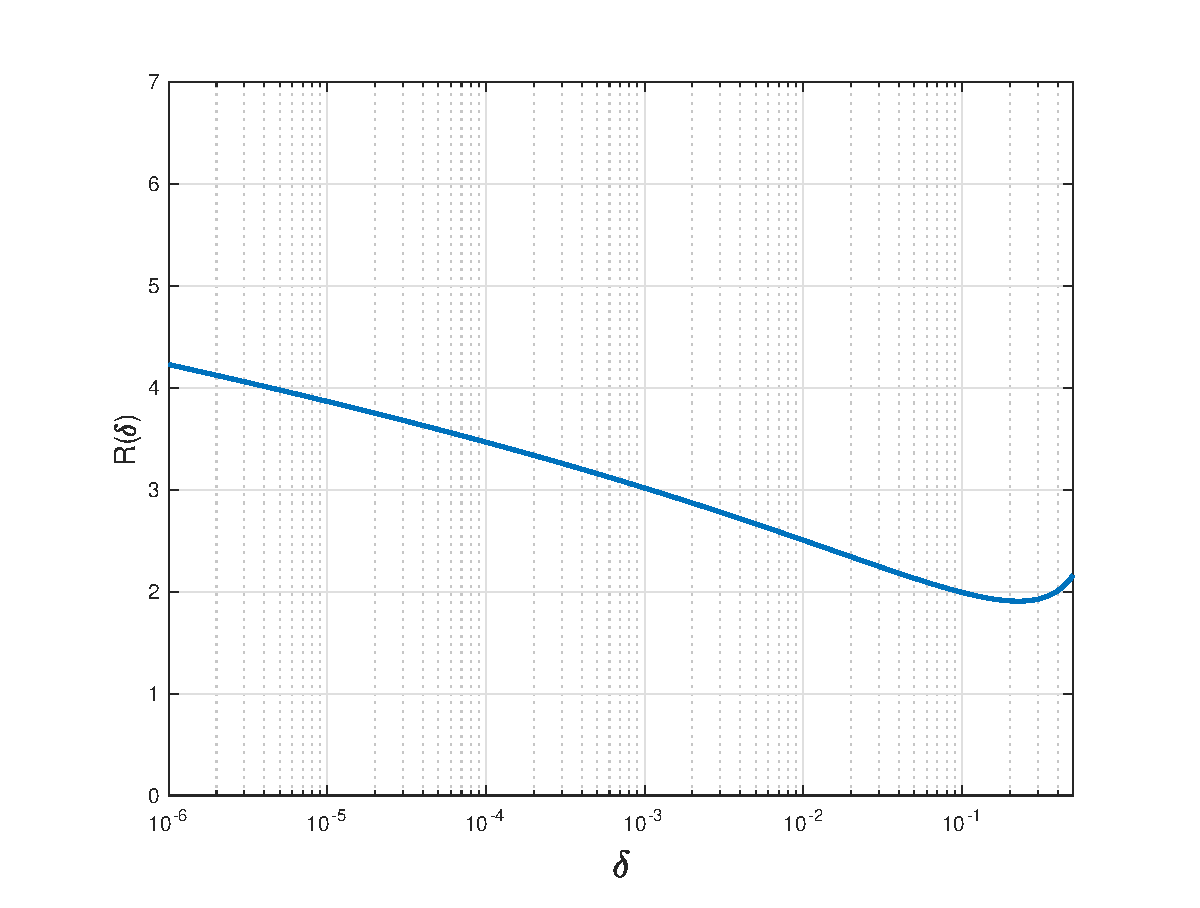
\includegraphics[width = 3in]{images/fig_1}\label{fig_1}} \hfil \subfigure[Low privacy regime.]{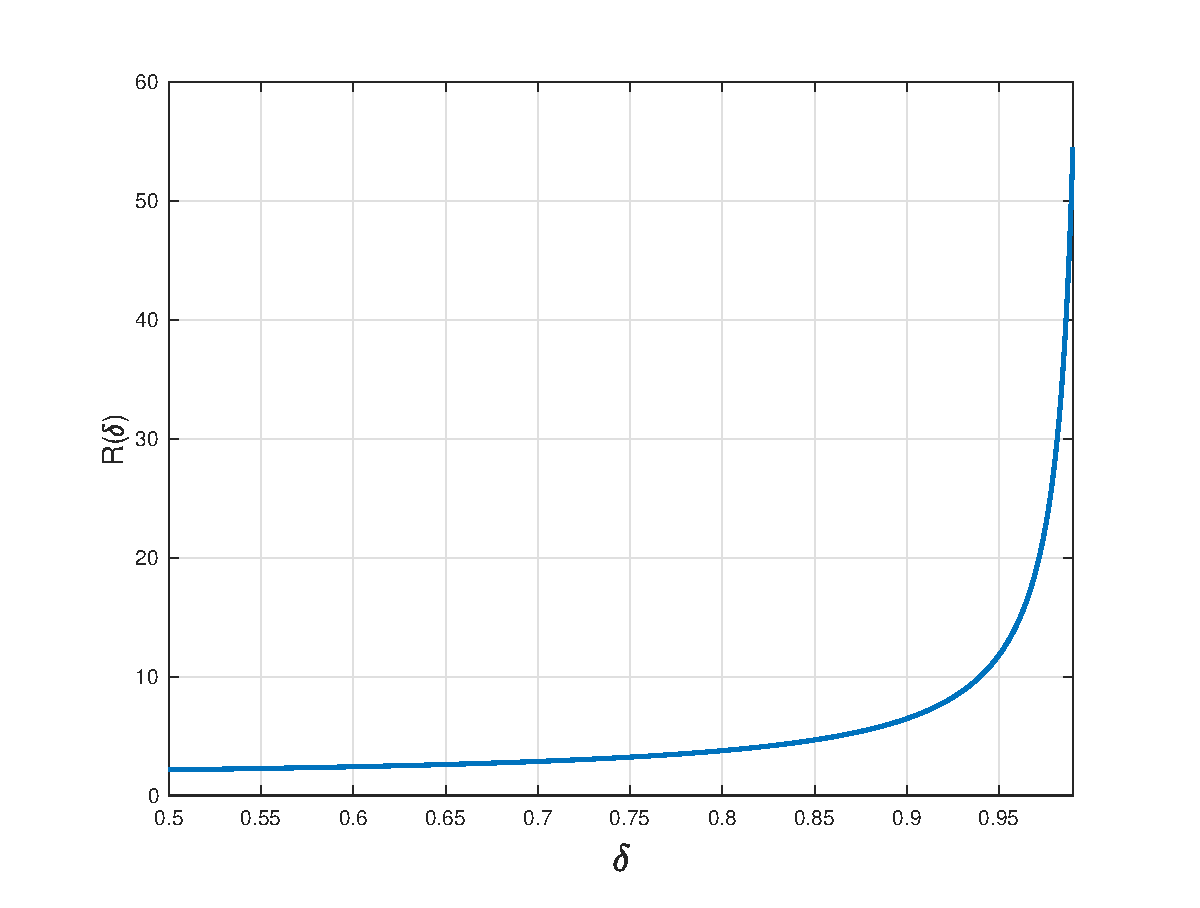
\includegraphics[width = 3in]{images/fig_2}\label{fig_2}}}
\caption{Ratio of expected noise magnitude of the classical Gaussian mechanism to that of optimal mechanism for $(\epsilon, \delta)$-differential privacy.}\label{fig_comparison}
 \end{figure*}  
It is observed in Fig.~\ref{fig_comparison} that noise magnitude reduction factor is increasingly more pronounced in the high privacy regime (i.e. low $\delta$), however, also shoots up in the low privacy regime as $\delta \rightarrow 1$. The optimal mechanism reduces the noise magnitude by more than $4$ times in the high privacy regime over the Gaussian mechanism.
%Need 2-3 pages on use case.
